\documentclass[format=sigconf]{acmart}
% \usepackage{usenix-2020-09}



\usepackage{enumitem}
\usepackage{subcaption}
% \usepackage{graphicx}
\usepackage{amsmath}
\usepackage{url}
\usepackage{color}
\usepackage{booktabs}
\usepackage{multirow}
\usepackage{tikz}
\usetikzlibrary{shapes.geometric,arrows,decorations.markings, arrows.meta}
\usetikzlibrary{positioning, calc}





% \raggedbottom
% 
\pagestyle{plain}
\begin{document}


\title{Attack Tree Edit Distance: refinement aware tree edit distance with semantic label replacement}

\iffalse{
    \author{Nathan D. Schiele}
    \orcid{0000-0003-1186-1503}
    \affiliation{\institution{Leiden University}
        \city{Leiden}
        \country{The Netherlands}}
    \email{n.d.schiele@liacs.leidenuniv.nl}


    \author{Olga Gadyatskaya}
    \orcid{0000-0002-3760-9165}
    \affiliation{\institution{Leiden University}
        \city{Leiden}
        \country{The Netherlands}}
    \email{o.gadyatskaya@liacs.leidenuniv.nl}
}\fi
\author{Anonymized for submission}




% \acmConference[FSE2024]{FSE2024}
% \acmYear{2024}
% %\acmBooktitle{Proceedings of the 32nd ACM Symposium on the Foundations of Software Engineering (FSE '24), November 15--19, 2024, Porto de Galinhas, Brazil}
% \acmBooktitle{Submission to FSE'24}

% \settopmatter{printfolios=true}

% \begin{teaserfigure}
%     \includegraphics[width=\textwidth]{img/Teaser02}
%     \caption{Participant created ADT}
%     \Description{A collage of ADTs that were created by participants}
%     \end{teaserfigure}

% \begin{teaserfigure}
% \includegraphics[width=\textwidth]{img/CollageTeaser}
% \caption{Assorted participant created ADTs}
% \Description{A collage of ADTs that were created by participants}
% \end{teaserfigure}


\begin{abstract}

    This is the abstract
\end{abstract}

\maketitle              % typeset the header of the contribution





\newcommand{\OG}[1]{{\color{blue} OG: #1}}
\newcommand{\NS}[1]{{\color{purple} NS: #1}}

\newcommand{\etal}{et al.}
\newcommand{\id}[2]{#1-#2}
\newcommand{\hypothesis}[1]{$\text{H}_\text{#1}$}
\newcommand{\RQ}[1]{\textbf{RQ#1}}

\newcommand{\ICS}{NCS}
\newcommand{\SEC}{CS}

\newcommand{\AND}{AND}
\newcommand{\SAND}{SAND}
\newcommand{\OR}    {OR}



\newcommand{\hypoCheckUnderstand}   {1}
\newcommand{\hypoSecondADT}         {2}
\newcommand{\hypoErrorAmount}       {3}
\newcommand{\hypoSelfUnderstand}    {4}
\newcommand{\hypoCommunicationTool} {5}
\newcommand{\hypoAnalysisTool}      {6}
\newcommand{\hypoWrittenComparison} {7}
\newcommand{\hypoIntentionToUse}    {8}
\newcommand{\hypoThirdADT}          {9}


\newcommand{\hypoMultipleParent}  {3-1}
\newcommand{\hypoMultipleRefinement}  {3-2}
\newcommand{\hypoMulipleCountermeasure}  {3-3}
\newcommand{\hypoSingleChildNodes}  {3-4}

\newcommand{\hypoGrades}            {10 - Not used}


\newcommand{\hResponse}[1]{\texttt{#1} - }

\newcommand{\anonfoot}{\footnote{Anonymized for submission}}


\newcommand{\qIndent}{4em}
\newcommand{\qsIndent}{2em}
\newcommand{\surveyq}[1]{\textbf{#1:}}

\section{Background}

Distance between data structures is not a new concept. Many works have explored the idea of ``distance'' between strings. In string edit distance, where the difference in strings is given my a min-cost path taken by either adding a character, removing a character or replacing a character. By fining the minimum cost needed to transform one string into another, a ``distance'' value can be given. As the higher cost a transformation, the further apart two strings must be \NS{cite all the string edit distance papers}.

Much of the work in this field has built upon work by Kuo-Chung Tai who suggested that the distance between trees is similar to several previous works comparing the differences in strings~\cite{tai_tree--tree_nodate}.

\section{Related Work}

Tree Edit Distance is not a new computational challenge. However, most of the development on tree edit distance focuses calculation optimization. As shown by Zhang~\etal, the tree edit distance problem for unordered trees is an \textit{NP}-Complete problem~\cite{zhang_editing_1992}. As such, the develop of novel optimal calculation strategies is necessary to enable comparison of larger tree structures. Zhang and Shasha proposed a commonly cited simple algorithm for calculating tree edit distance~\cite{zhang_simple_1989}. We use this algorithm in this paper as it is a common strategy for implementing and testing extensions to tree edit distance. As such, optimizations based on the Zhang and Shasha algorithm can be applied to our methodology as we show in section \NS{When I write that section, I'll reference it here}.

Tree edit distance, like string edit distance, has a wide array of applications. Just as string edit distance has been used to compare sequences of DNA \NS{cite},

\section{Refinement Awareness}

One of the biggest differences between attack trees and other tree-like data structures is the presence of refinements, or the \AND\ and \OR\ relationships, which state whether all of the children of a node must be satisfied for the parent node to be satisfiable (\AND) or if at least one must be satisfied for a parent node to be satisfiable (\OR).

The presence of refinements in a tree does not significantly complicate the calculation of tree edit distance. As given by RTED?, the tree edit distance can be given by the summation: \NS{include the nice summation from whatever paper I think I saw it in}.

In the Zhang and Shasha algorithm there are three possibilities for nodes, (i) a node must be added, (ii) a node must be removed, or (iii) a node must be replaced. Assume for each case that the resulting refinement must also be changed. If the cost of this change is given to be $\gamma(\Delta)$, then this cost would be applied to all three cases. As such, the min-cost calculation is given as follows:

\begin{equation*}
    \text { forestdist }\left(l\left(i_1\right) \ldots i, l\left(j_1\right) . . j\right)=\min \left\{\begin{array}{l}
        \text { forestdist }\left(l\left(i_1\right) \ldots i-1, l\left(j_1\right) . . j\right)+\gamma\left(T_1[i] \rightarrow \Lambda\right), \\
        \text { forestdist }\left(l\left(i_1\right) . . i, l\left(j_1\right) . . j-1\right)+\gamma\left(\Lambda \rightarrow T_2[j]\right),    \\
        \text { forestdist }\left(l\left(i_1\right) . . l(i)-1, l\left(j_1\right) . . l(j)-1\right)                                           \\
        + \text { forestdist }(l(i) \ldots i-1, l(j) . . j-1)                                                                                 \\
        +\gamma\left(T_1[i] \rightarrow T_2[j]\right) .
    \end{array}\right.
\end{equation*}

Which would subsequently be equal those

\NS{give min cost calculation with the $\gamma(\Delta)$ on the outside}

As the cost of replacing refinements is ever present, we can simply apply the cost of the replacing refinements after computing the tree edit distance by following the mappings and subsequently applying changed refinements. By doing this, we do not add to the time complexity of the Zhang and Shasha algorithm.

This method of computation works as it is not possible to have an intermediate attack tree node without a refinement~\cite{mauw_foundations_2006}. As such, all non-leaf nodes are either \AND\ or \OR\ nodes, so the distance between refinements is simple given as the cost needed to convert from one refinement to the other. As unlike the calculations of adding ($\Lambda \rightarrow i$), removing ($i \rightarrow \Lambda$), or replacement ($i \rightarrow j$), with refinements there is only on possible operation: replacement. Either \AND $\rightarrow$ \OR\ or \OR $\rightarrow$ \AND.

Similarly, \NS{the binary trees people}

Critically, this methodology can only work so long as the order of the nodes does not carry any significance (\textit{i.e} the nodes can be reordered without issue). There is an extention of attack trees which adds a sequential \AND\ (\SAND) refinement, in which the nodes in a \SAND\ relationship are given to be ordered~\cite{jhawar_attack_2015}; however, this is out of scope for our purposes. We discuss this further in Section~\NS{ref future work}.
\section{Semantic Label Replacement}

In tree edit distance, the replacement calculation is made when the root nodes of subtrees are not the same~\cite{zhang_simple_1989}. Prior to calculation, a mapping is made between all nodes with the same labels, and this mapping is used to determine equivalence of nodes within the two trees. The labels of these nodes are typically given to be capital letters of the alphabet. However, in practical application, node labels are typically significantly more complex than mere letters.

One approach would be to ignore labels entirely.


\subsection{Semantic comparison}


\subsection{Semantic mapping}

As such, we introduce a new mapping step.

The steps:
\begin{enumerate}
    \item determine semantic cut off value $\epsilon$
    \item list all node labels between both trees
    \item calculate the semantic similarity between all node labels between the two trees
          \begin{itemize}
              \item this is given by comparing semantic embeddings
              \item This is a value between 0 and 1, with 0 being no semantic similarity and 1 being identical semantic similarity
          \end{itemize}
    \item starting with node labels with the highest semantic similarity
    \item remove these labels from both lists
    \item repeat until at least one list is empty, or all semantic similarity values are below $\epsilon$
\end{enumerate}

After performing this mapping step, we compute tree edit distance as described by Zhang and Shasha. However, the cost of replacing a node with another node is given as 1 - semantic similarity. In this way, nodes that have highly similar labels (a semantic similarity approaching 1) will have a low replacement cost, while those with little to no semantic similarity will have high replacement cost. Additionally, if we give that the cost of adding or removing a node to be 1, we prime the Zhang and Shasha algorithm to attempt to replace as many nodes as possible. \NS{this may not be a good thing}


\section{Node Flipping}

The Zhang and Shasha edit distance algorithm is specifically given for ordered trees, that is, the order of child nodes is taken to be significant. In attack trees without sequential conjunction, the order of nodes is not given to be significant~\cite{mauw_foundations_2006,jhawar_attack_2015}. This results in an issue where trees with identical, but unordered nodes are given to have a high edit distance. This is shown in Figure~\ref{fig:nodeflipping}, where two trees with identical information but different node order are given to have a distance of 2. This is due to the fact that the Zhang and Shasha algorithm is not designed to handle unordered trees. 


\begin{figure}
    \begin{subfigure}{.45\linewidth}
        \includegraphics[width=\linewidth]{img/NodeFlip1.png}
    \end{subfigure}
    \begin{subfigure}{.45\linewidth}
        \includegraphics[width=\linewidth]{img/NodeFlip2.png}
    \end{subfigure}
    \caption{Two attack trees (subtrees of the example in Figure~\ref{fig:tartgetAT}) with identical information but different node order. These trees would evaluate to have a distance of 2 (two replacement operations).}
    \label{fig:nodeflipping}
\end{figure}




\subsection{Semantic mapping}

% Prior to calculation, a mapping is made between all nodes with the same labels, and this mapping is used to determine equivalence of nodes within the two trees. The labels of these nodes are typically given to be capital letters of the alphabet. However, in practical application, node labels are typically significantly more complex than mere letters.

% We introduce a new mapping step. As attack trees without sequential conjunction (\SAND\ refinements) are generally given to be unordered, we must implement an unordered semantic mapping. As described by Paa{\ss}en builds upon the work Zhang~\etal\ described for

% The steps:
% \begin{enumerate}
%     \item determine semantic cut off value $\epsilon$
%     \item list all node labels between both trees
%     \item calculate the semantic similarity between all node labels between the two trees
%           \begin{itemize}
%               \item this is given by comparing semantic embeddings
%               \item This is a value between 0 and 1, with 0 being no semantic similarity and 1 being identical semantic similarity
%           \end{itemize}
%     \item starting with node labels with the highest semantic similarity
%     \item remove these labels from both lists
%     \item repeat until at least one list is empty, or all semantic similarity values are below $\epsilon$
% \item Once we have our mappings, we reorder siblings as best as possible
% \begin{enumerate}
%     \item Starting with leaves, siblings can be swapped for no cost
%     \item Done if it improves the mapping
%     \item \textit{may result in local minima issues - but will be optimal enough}
% \end{enumerate}
% \end{enumerate}
\section{Experimental methodology}

We evaluated our results using study data from a study that was performed with student participants.

\subsection{Participants}
The participants in this study were all third year bachelor students taking part in a minor on cyber security and governance. Most students were in policy related majors such as Security Studies or International Relations. The participants on average had only a few months of programming experience, which was a result of another course in the minor. Students were asked if they had any prior knowledge of threat models or attack trees, and only a few students had any prior knowledge. Students took this course in the fall semester of 2023. As shown by Naiakshina~\etal\ and Karpati~\etal, in the context of cyber security, students are a sufficient proxy for practitioners~\cite{karpatiComparingAttackTrees2014, naiakshinaConductingSecurityDeveloper2020}.

\subsection{Study design}

Students were assigned a project related to attack defense trees as a part of their regular coursework. The project was a mandatory, graded assignment. Students had the option to provide consent for their anonymized responses to be collected for research purposes, this is described in detail in Section~\ref{ssec:ethics}. The assignment consisted of four components. In each component, students were required to create an attack (defense) tree (ADT) using a web application of our own design. Of the four components, the third was included in the assignment for the purposes of validating our approach. The text of the entire study is included in Appendix~\NS{INCLUDE}; however, we only expound upon the relevant section in this work.

The third component of the study contains two parts. In part A, students were tasked with creating an AT from a provided, written, scenario. The scenario was adapted from an attack tree shown in Naik~\etal~\cite{naikEvaluationPotentialAttack2022}. The scenario was as follows:

\texttt{Many attackers aim to obtain personal data. Gathering personal data can be completed through unauthorized access to profile, credential creep, or a background data attack. Unauthorized access to profile requires gaining user credentials and accessing the profile. The credentials can be gained through a malware attack or a social engineering attack, and the profile can be accessed by stealing a phone or by remote access. Credential creep can be completed by submitting a request for additional data other than what is needed for verification or by user profiling. Finally, a background data attack requires both obtaining a sensitive dataset and linking the dataset via a request for verification.}

This description was created by reading the attack tree in Naik~\etal\ abstraction level by abstraction level, always going from left to right. 

We then asked students in part B to expand upon their attack tree by ``doing your own research, add at least 5 new nodes and 2 new refinements to the attack tree you created in the previous section''. In all, this creates a relatively predictable, yet varied, dataset. In Part A, all trees should roughly be the same, baring minor changes in the label of nodes or the order of nodes. We expect that any large differences in part A to be due to misunderstanding the assignment or misreading the scenario. As Part B is built from each students' part A, we expect that the ``core'' of their attack tree to remain unchanged but the added nodes and refinement should introduce an ability to evaluate edit distance. Based on previous experience with similar studies, we expect most students to add exactly 5 new nodes and 2 new refinements, which should allows for some predictable edit distance (namely, the cost of adding 5 new nodes).

\subsubsection{Web application}

For this assignment, we created a web application which can be used to create attack defense trees. The web application contains a graphic interface with which users can add, delete and modify nodes~\cite{mohalaiaImplementingUserInterface2023}. Additionally, the web application contains an SQL-like language that can be used to generate ADTs~\cite{mezaADTLangDeclarativeLanguage2023}. The Web application additionally allows users to download ADTs as images as well as in the ADTool XML schema as defined by Kordy~\etal~\cite{kordy_adtool_2013}. The web application can be found here: \url{https://nschiele.github.io/ADT-Web-App}.

\subsection{Processing}

The attack tree data was collected in the form of XML data. This data was then processed using a Python script. The script was used to extract the attack trees from the XML data and to convert the attack trees into a format that could be used by our implementation of the Zhang and Shasha algorithm. We started with the pre-implemented and tested \texttt{zss} library from Tim Henderson~\cite{hendersonZssTreeEdit}. We then modified the library to include our semantic label replacement cost, refinement chang cost, and our abstraction layer-wise semantic node flipping to create an implementation of the Zhang and Shasha algorithm that should be effective for attack trees. We subsequently used this implementation to calculate the tree edit distance between the attacks trees. Our code is provided here: \url{http://}\NS{link.to.github?}.


\subsection{Ethics}
\label{ssec:ethics}
This study was approved by the the Ethics Review Board at a european university\anonfoot. Students were informed of study and were requested to give consent for their responses to be included in the study. Multiple safeguards were used to ensure that students did not feel pressured into giving consent, as the assignment was a mandatory course component. Students were informed that they could withdraw their consent at any time, and that their responses would be anonymized. 




\section{Results}
\label{sec:results}



\subsection{Measuring $\gamma(\Delta)$}

\NS{Operations plot}

\NS{plot showing the effect of refinement costs}

\subsection{Finding optimal $\epsilon$}

In Figure~\ref{img:similaritylimits}, we can see the effect of rising semantic similarity limit ($\epsilon$) on the average distance between each of attack tree 1 ($n=38$). Additionally, we can see the normalized Levenshtein distance plotted against the same semantic similarity limits. Finally, we can see the traditional Zhang and Shasha edit distance (based on string equivalence), which is unaffected by a similarity limit.

\begin{figure}
    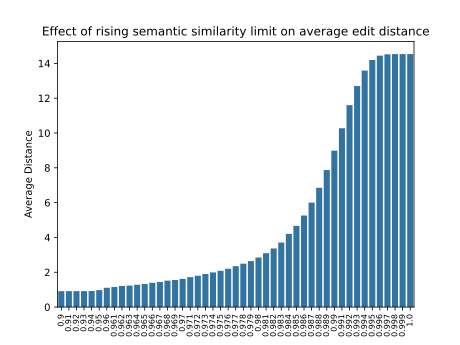
\includegraphics[width=\linewidth]{code/img/similaritylimits.pdf}
\caption{The average distance between the 38 experimental ATs per semantic similarity limit}
\label{img:similaritylimits}
\end{figure}

\NS{Operations plot}


\section{Effect of node flipping}

\NS{plot showing average distance between 38 ATs with and without node flipping}




\cite{*}



\bibliography{bibliography}{}
\bibliographystyle{plain}



\appendix
% \section*{Appendix}

\subsection{Operations table for counterexamples}
\begin{table*}
    \resizebox{\textwidth}{!}{
        \begin{tabular}{lcccccccccccccccc}
            \toprule
            Counterexample       & \multicolumn{4}{|c|}{Label Distance} & \multicolumn{4}{|c|}{Tree Edit Distance} & \multicolumn{4}{|c|}{Radical Distance} & \multicolumn{4}{|c|}{Multiset Distance}                                                                                                 \\
                                 & Remove                               & Add                                      & Change                                 & Match                                   & Remove & Add & Change & Match & Remove & Add & Change & Match & Remove & Add & Change & Match \\
            \midrule
            Order Reversed       & 0                                    & 0                                        & 0                                      & 7                                       & 0      & 0   & 6      & 1     & 0      & 0   & 0      & 7     & 0      & 0   & 0      & 4     \\
            Refinement Switch    & 0                                    & 0                                        & 0                                      & 7                                       & 0      & 0   & 2      & 5     & 0      & 0   & 2      & 5     & 1      & 1   & 1      & 2     \\
            Extra Intermediate   & 1                                    & 0                                        & 0                                      & 7                                       & 1      & 0   & 0      & 7     & 1      & 0   & 0      & 7     & 0      & 0   & 0      & 4     \\
            Missing Intermediate & 0                                    & 1                                        & 0                                      & 6                                       & 0      & 1   & 0      & 6     & 1      & 3   & 0      & 4     & 0      & 0   & 0      & 4     \\
            Extra Leaf           & 1                                    & 0                                        & 0                                      & 7                                       & 1      & 0   & 0      & 7     & 1      & 0   & 0      & 7     & 1      & 0   & 0      & 4     \\
            Missing Leaf         & 0                                    & 1                                        & 0                                      & 6                                       & 0      & 1   & 0      & 6     & 0      & 1   & 0      & 6     & 0      & 1   & 0      & 3     \\
            Changed Root         & 0                                    & 0                                        & 1                                      & 6                                       & 0      & 0   & 1      & 6     & 0      & 0   & 1      & 6     & 0      & 0   & 0      & 4     \\
            Changed Intermediate & 0                                    & 0                                        & 1                                      & 6                                       & 0      & 0   & 1      & 6     & 0      & 0   & 1      & 6     & 0      & 0   & 0      & 4     \\
            Changed Leaf         & 0                                    & 0                                        & 1                                      & 6                                       & 0      & 0   & 1      & 6     & 0      & 0   & 1      & 6     & 0      & 0   & 1      & 3     \\
            Move Adjacent        & 0                                    & 0                                        & 0                                      & 7                                       & 1      & 1   & 0      & 6     & 1      & 1   & 0      & 6     & 1      & 2   & 0      & 2     \\
            Move Up              & 0                                    & 0                                        & 0                                      & 7                                       & 1      & 1   & 0      & 6     & 1      & 1   & 0      & 6     & 0      & 0   & 0      & 4     \\
            Move Down            & 0                                    & 0                                        & 0                                      & 7                                       & 1      & 1   & 0      & 6     & 2      & 1   & 0      & 5     & 0      & 1   & 0      & 3     \\
            \bottomrule
        \end{tabular}

    }
    \caption{Table showing the operations per counterexample and distance measure}
\end{table*}

% \appendix
% \input{content/questionnaire}

\end{document}
